\subsubsection{CountMin\cite{cormode_improved_2003}}

\paragraph{}
CountMin could be considered as the pioneering work in summarizing data streams which are directly related to our research. CountMin is a data structure that is used for frequency approximation queries. The underlying idea behind the CountMin data structure is to hash the aggregated frequencies of the edges using multiple hash functions into predefined blocks as indicated in \autoref{fig:countmin}. A fixed-size will be stated at the time of the creation of the CountMin sketch and irrespective of the volume of data stored, the size of the sketch does not have to be changed. The major drawback in following this procedure is that the error of the queries reduce as more and more data is introduced to the sketch. However, despite these weaknesses, CountMin can be considered as a good generalized sketch at the time as many other sketches described in the literature are good for one single pre-specified aggregate computation. Therefore CountMin approach is not restricted to streaming graphs but other applications as well\cite{cormode_improved_2003}.

\begin{figure}[H]
    \centering 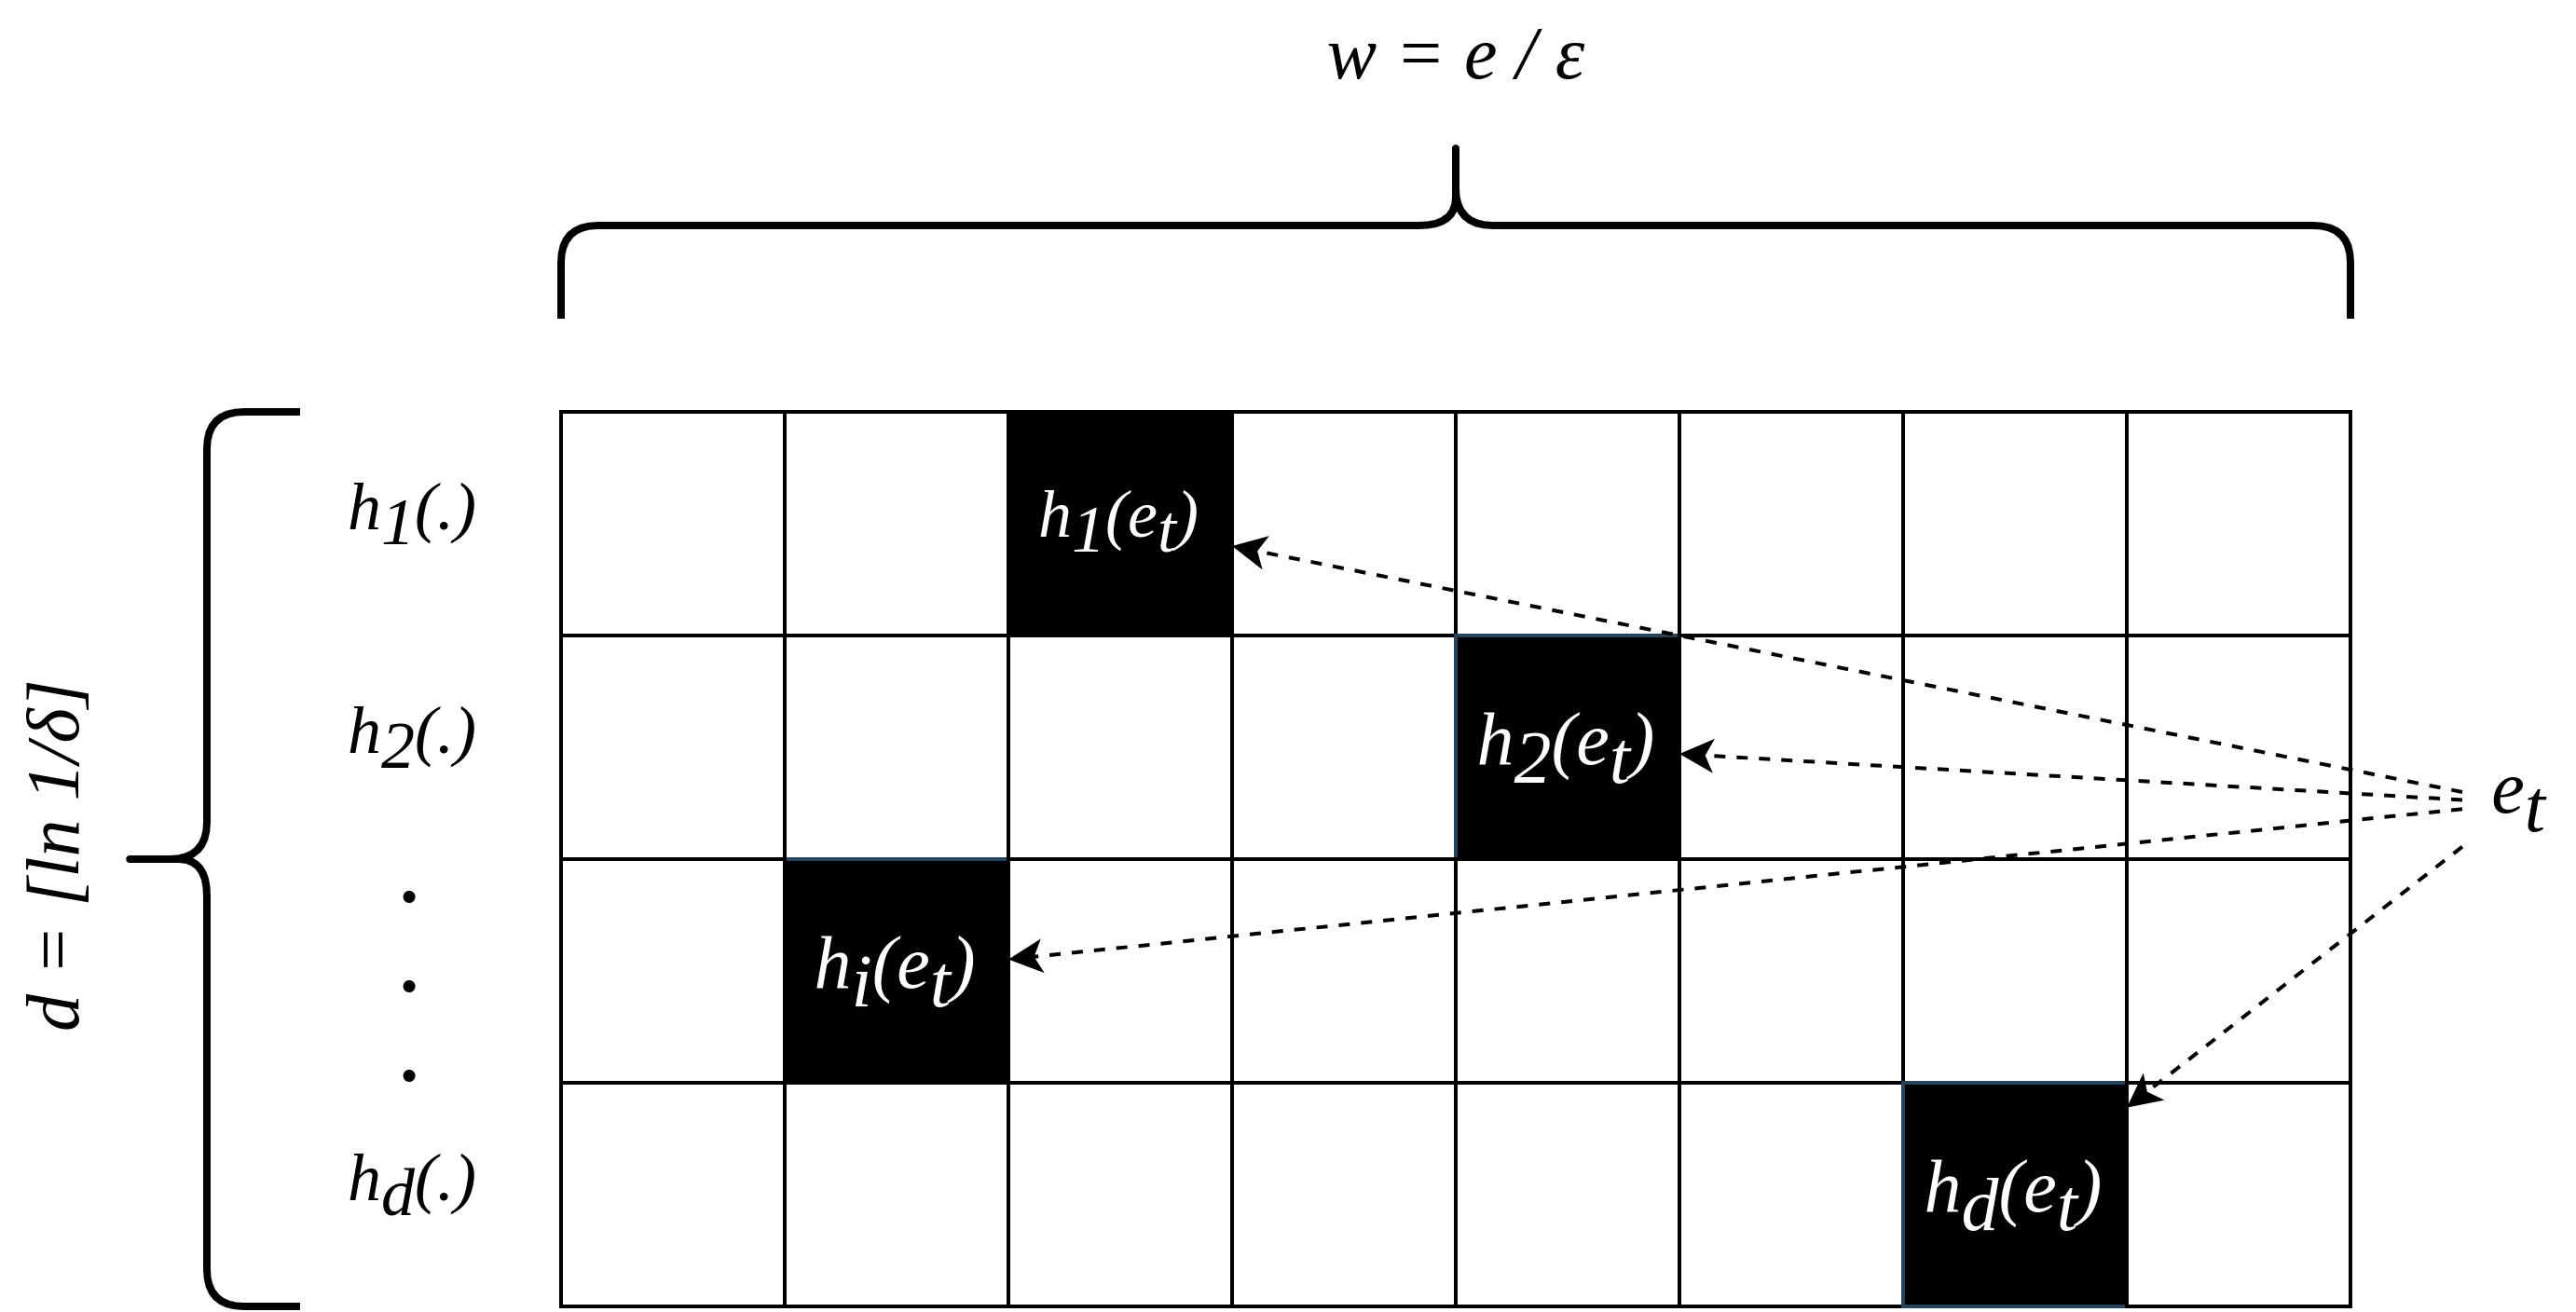
\includegraphics[width=\textwidth]{countmin}
    \caption{CountMin sketch}
    \label{fig:countmin}
\end{figure}